\chapter{Implementierung}\label{ch:implementierung}
Das folgende Kapitel beschreibt die eigene Entwicklung einer Indexstruktur zur Optimierung der \textit{k}-Nächsten-Nachbarn-Suche nach Bloom-Filtern in AMBIENCE. Sie heißt \textit{BloomFilterTree}. Abschnitt \ref{sec:aufbau} stellt den konzeptionellen Aufbau dar. Die praktische Umsetzung wird in Abschnitt\ref{sec:umsetzung} beschrieben. Die zentralen Operationen zum Einfügen von Bloom-Filtern und die \textit{k}-nächste-Nachbarn-Suche werden in den Abschnitten \ref{sec:einfügen} und \ref{sec:knn} vorgestellt. Abschließend wird erläutert, welche alternativen Ansätze während der Implementierung verfolgt und aus welchen Gründen sie letztlich verworfen wurden (vgl. Abschnitt \ref{sec:alternativen}). Die Evaluation des Verfahrens und Gegenüberstellung mit der naiven Implementierung ist im folgenden Kapitel \ref{ch:evaluation} zu finden.  
\section{BloomFilterTree}\label{sec:bloom-filter-tree}
Um möglichst plattformunabhängig zu bleiben, wurde die Implementierung in C++ realisiert. Ausgewählte Codebeispiele finden sich im Anhang (vgl. Kapitel \ref{ch:anhang}).  
\subsection{Aufbau}\label{sec:aufbau}
Wie in Kapitel \ref{ch:related} dargestellt, diente die Arbeit von Sakuma und Sato über "`Structured Bloom Filters Based on Similarity"' zunächst als Grundlage\footnote{Vgl. \cite{Sakuma2011}.} für die Indexstruktur. Zur Organisation der Bloom-Filter wurde zuerst ein B$^+$-Baum implementiert mit allen Eigenschaften wie in Abschnitt \ref{sec:indexstrukturen} beschrieben. Dieser wurde schrittweise für die Verwendung mit Bloom-Filtern erweitert: 
\begin{enumerate}
	\item Die Datensätze sind Bloom-Filter, d.h. die jedes Blatt enhält Zeiger auf die \textit{n} Bloom-Filter-Objekte, die darin eingefügt wurden. Bloom-Filter-Objekte werden über ihre ID als Primärschlüssel identifiziert. 
	\item Jeder Baumknoten hat einen Vereinigungsfilter. Er wird aus dem bitweisen logischen Oder aller Bloom-Filter gebildet, die in den darunter liegenden Teilbaum eingefügt wurden (vgl. Abschnitt \ref{sec:bloom-index}).
\end{enumerate}
Abb. \ref{fig:pic6} veranschaulicht den Aufbau eines BloomFilterTree. Die Baumknoten sind darin blau markiert. Sie enhalten die Primärschlüssel der Bloom-Filter sowie Zeiger auf die Kind- bzw. Nachbarknoten. Jeder Knoten hat einen Vereinigungs-Bloom-Filter, der weiß markiert ist. Die tatsächlichen Datensätze sind violett markierte Bloom-Filter. Die Blätter des BloomFilterTree verweisen jeweils auf die darin eingefügten Datensätze.
\newpage
\begin{figure}[hpbt]
  \centering
  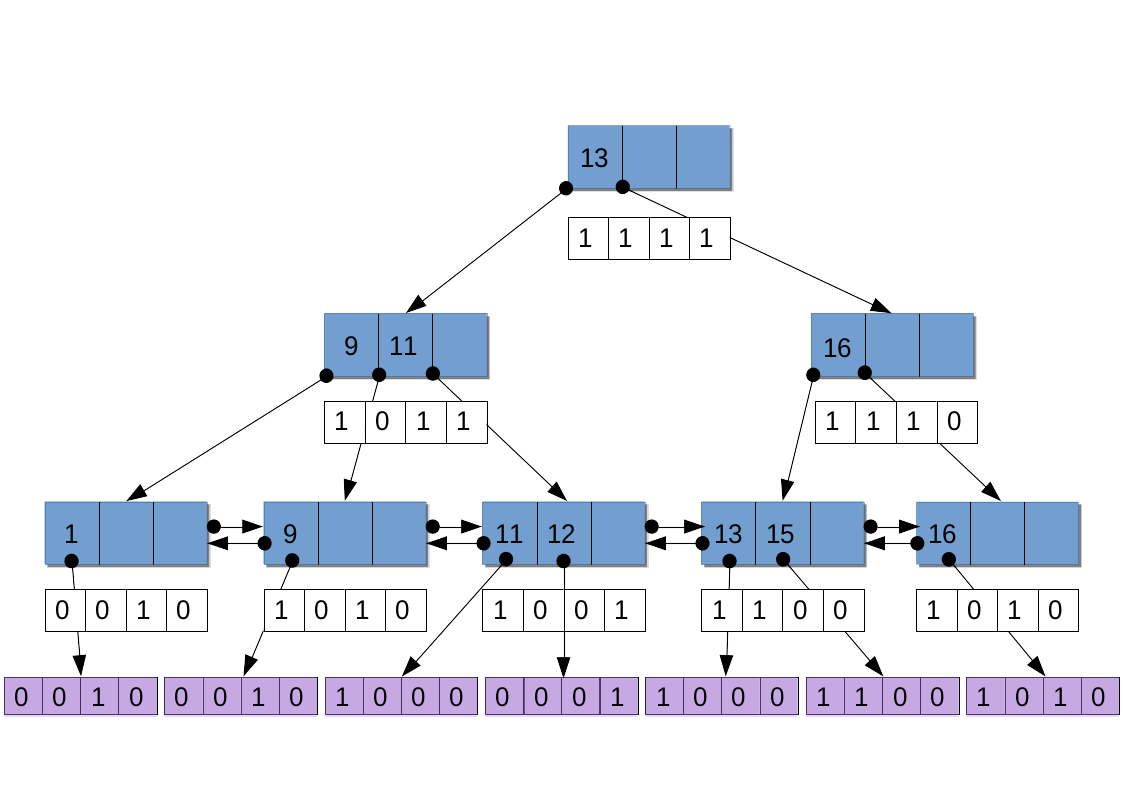
\includegraphics[width=1.0\textwidth]{pictures/bloom-filter-tree.png}\\
  \caption[Aufbau eines BloomFilterTree]{Aufbau eines BloomFilterTree mit Bloom-Filtern als Datensätzen und Vereinigungsfiltern an allen Knoten.}\label{fig:pic6}
\end{figure}
\subsection{Umsetzung}\label{sec:umsetzung}
Die Klasse \textit{BloomFilterTree} enthält schließlich alle notwendigen Parameter und Operationen zur Organisation der Bloom-Filter. Dazu gehören die B$^+$-Baum-Operationen wie Einfügen und Suchen von Schlüsseln, Traversieren der Blätter, boolesche Abfrage nach Enthaltensein eines Schlüssel im Baum, Zählen der Blätter und viele mehr. Darüber hinaus enthält die Klasse:  
\begin{enumerate}
	\item \textit{Management-Methoden} zum Berechnen der Jaccard-Distanzen zu allen Filtern im Baum, k-Nächste-Nachbarn-Suche in der naiven Version, Traversieren der Datensätze (also der Bloom-Filter) etc..
	\item Die \textit{zentralen Methoden} des Verfahrens: Einfügen der Bloom-Filter nach Ähnlichkeit und die \textit{k}-Nächste-Nachbarn-Suche. 
	\item \textit{Methoden für Messungen und Vergleich} von Werten, z.B. für die verschiedenen Varianten der \textit{k}-Nächste-Nachbarn-Suche, die Aufbaukosten und den Speicherbedarf der Datenstruktur. 
\end{enumerate}
Die Header-Datei der Klasse BloomFilterTree ist im Anhang abgedruckt (vgl. Abschnitt \ref{sec:BloomFilterTree.hpp}).

Die Klasse \textit{BloomFilter} enthält alle wichtigen Parameter und Operationen auf Bloom-Filtern, also unter anderem: 
\begin{enumerate}
	\item \textit{Typische Bloom-Filter-Parameter und -Methoden} wie Anzahl der Hashfunktionen, Daten-Array und Setzen von Bits.
	\item \textit{Mathematische Methoden und Vergleichsoperationen} wie Berechnung von Teil- und Obermengen, bitweises logisches Und und Oder, Berechnung und Abschätzung der Jaccard-Distanz etc..
	\item \textit{Methoden zum Bloom-Filter-Management} wie Einfügen von zufälligen Elementen aus einem Wörterbuch, zufällige Initialisisierung mit Werten aus $\{0,1\}$ usw..
\end{enumerate}
Die Header-Datei der Klasse BloomFilterTree ist im Anhang abgedruckt (vgl. Abschnitt \ref{sec:BloomFilter.hpp}).
\subsection{Einfügen}\label{sec:einfügen}
Das Verfahren zum Einfügen zählt zu den wichtigsten Methoden der Indexstruktur und ist entscheidend für die Optimierung von Laufzeit und CPU-Zeit der k-Nächste-Nachbarn-Suche. Der Algorithmus basiert auf den Teil- und Obermengenbeziehungen zwischen Bloom-Filtern und nutzt die Vereinigungsfilter der bereits existierenden Knoten, um die optimale Position zum Einfügen eines neuen Bloom-Filters in den BloomFilterTree zu finden. Er besteht aus folgenden Schritten: 
\begin{enumerate}
	\item Falls der Baum noch leer ist: Erstelle einen neuen Blattknoten und füge das Bloom-Filter-Objekt als erstes Datenobjekt ein. Der neue Knoten ist die Wurzel des BloomFilterTree.  
	\item Andernfalls suche ausgehend vom Wurzelknoten rekursiv die optimale Position im Baum: 
	\begin{enumerate}
		\item % TODO 
	\end{enumerate}
\end{enumerate}
\subsection{k-Nächste-Nachbarn-Suche}\label{sec:knn}
\section{Alternative Ansätze}\label{sec:alternativen}
\subsection{Einfügen gemäß Jaccard-Distanzen}\label{sec:ähnlichkeit}
\subsection{Doppelt verkettete Liste}\label{sec:verkettete-liste}
%%Es lassen sich auch mehrere Bilder nebeneinander platzieren wie z.B. in Abbildung
%%\ref{fig:multipic} zu sehen ist.
%%\begin{figure}[hpbt]
%% \centering
%%  %%----start of first subfigure----
%%  \subfloat[FIFO size limited to 20 entries]{
%%   \label{fig:multipic:a} %% label for first subfigure
%%   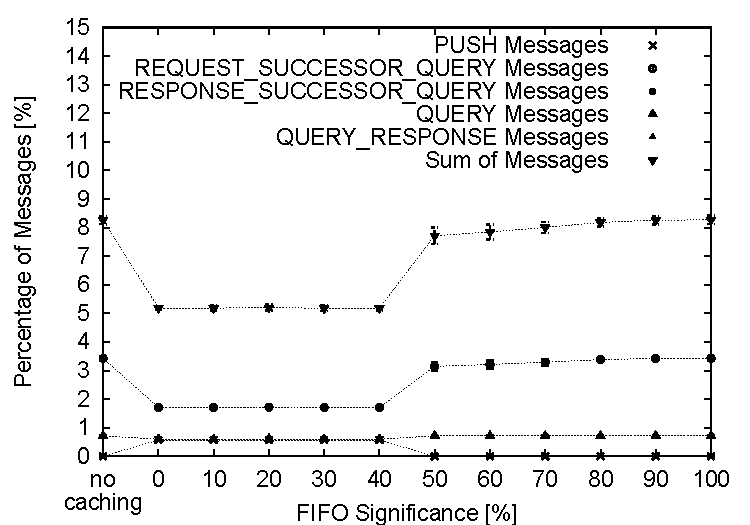
\includegraphics[width=0.48\linewidth]{pic1}}
%%  \hspace{0.01\textwidth}
%%  %%----start of second subfigure----
%%  \subfloat[FIFO size limited to 30 entries]{
%%   \label{fig:multipic:b} %% label for second subfigure
%%   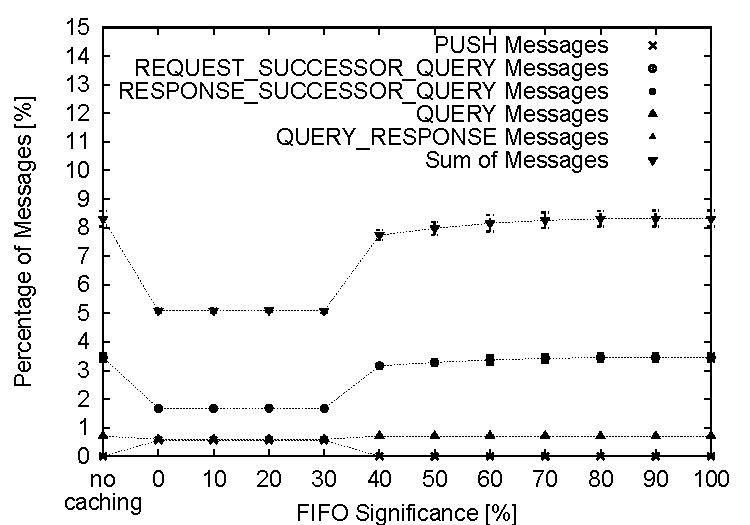
\includegraphics[width=0.48\linewidth]{pic2}}\\[0pt] % horizontal break
%%  %%----start of third subfigure----
%%  \subfloat[FIFO size limited to 40 entries]{
%%   \label{fig:multipic:c} %% label for third subfigure
%%   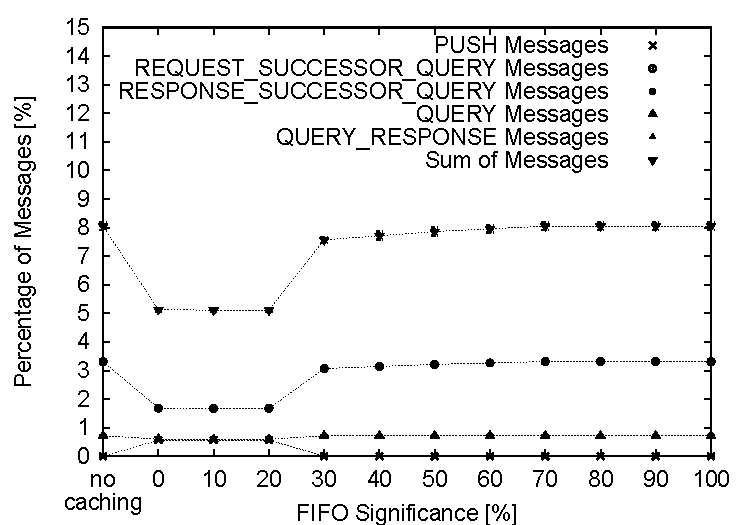
\includegraphics[width=0.48\linewidth]{pic3}}
%%  \hspace{0.01\textwidth}
%%  %%----start of fourth subfigure----
%%  \subfloat[FIFO size limited to 50 entries]{
%%   \label{fig:multipic:d} %% label for fourth subfigure
%%   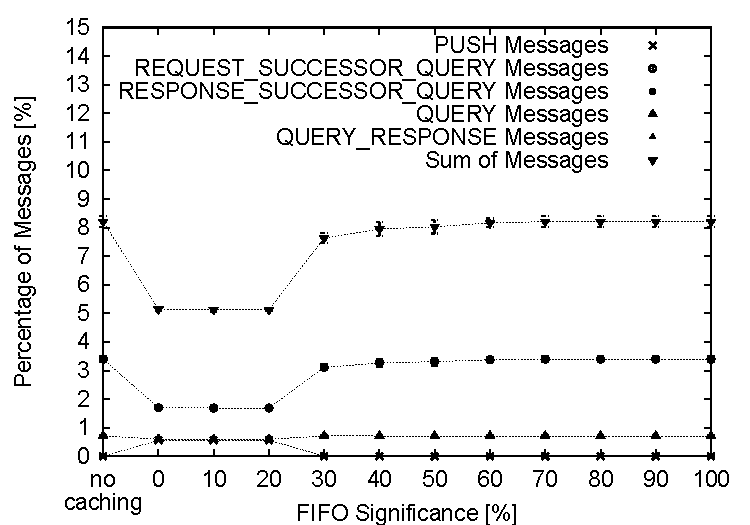
\includegraphics[width=0.48\linewidth]{pic4}}
%% \caption[Observed message fractions and 95\% confidence intervals for Chord]{Observed message fractions and 95\% confidence intervals for Chord without the influence of churn. The FIFO capacity varies from 20 (\ref{fig:multipic:a}) -- 50 (\ref{fig:multipic:d}) entries (decadic steps).}
%% \label{fig:multipic} %% label for entire figure
%%\end{figure}
%%
%%\subsection{Programm Code}
%%Eine elegante Möglichkeit, Programmtext einzubinden, lässt sich mit dem listings-Paket erreichen.
%%Das \verb|HelloWorld| Programm aus Listing \ref{lst:hw} hat in Zeile \ref{line:hw3} übrigens einen Programmierfehler.
%%\begin{lstlisting}[float=htp,caption=Hello World,label=lst:hw,language=Java, numbers=left, numberstyle=\tiny, stepnumber=2, numbersep=8pt, escapeinside={//@}{@//},backgroundcolor=\color{yellow},xleftmargin=3ex,xrightmargin=1ex]
%%public class HelloWorld {
%%    public static void main(String[] args) {
%%        Syste.out.println("Hello, World"); //@\label{line:hw3}@//
%%    }
%%}
%%\end{lstlisting}
%
